\documentclass[preprint,12pt,authoryear]{elsarticle}

\usepackage{amsmath,amssymb,amsfonts}
\usepackage{booktabs}
\usepackage{graphicx}
\usepackage{float}
\usepackage{placeins}
\usepackage{hyperref}
\usepackage{lineno}

\linenumbers

\journal{Energy and AI}

\begin{document}

\begin{frontmatter}

\title{Operational Diversity by Design: A Parametric Simulation Methodology for Zero-Shot Building Load Forecasting}

\author[smu]{Jeong-Uk Kim\corref{cor1}}
\ead{jukim@smu.ac.kr}
\cortext[cor1]{Corresponding author}

\affiliation[smu]{organization={Department of Electrical Engineering, Sangmyung University},
            city={Seoul},
            postcode={03016},
            country={South Korea}}

\begin{highlights}
\item 700 designed simulations approach 900K stock-model zero-shot performance
\item Coverage-based framework interprets why design can substitute for scale
\item LHS shows 1.33 pp gain over one equal-size stock-model control
\item RevIN benefit is regime-dependent: helps designed, hurts stock data
\item Full pipeline runs in under one day on a single workstation
\end{highlights}

\begin{abstract}
Zero-shot building load forecasting requires simulation datasets that capture diverse real-world operational patterns. Existing approaches rely on large building-stock databases containing hundreds of thousands of buildings, but the relationship between dataset design and zero-shot generalization remains poorly understood. This paper develops a coverage-based interpretation of the Operational Diversity Hypothesis: zero-shot transfer appears to depend not only on sample count, but also on how broadly the training set spans the operational parameter space.

We define a 12-dimensional operational schedule space --- spanning operating hours, baseload behavior, equipment retention, weekly disruptions, seasonal variation, and stochastic noise --- and use it to motivate four empirical expectations about the advantage of design-based sampling over stock-model sampling, the onset of N-scaling plateaus, the regime-dependent effect of Reversible Instance Normalization (RevIN), and the failure mode on out-of-scope building types.

We instantiate this interpretation through 700 EnergyPlus simulations (50 per archetype $\times$ 14 types) with Latin Hypercube Sampling, combined with RevIN and data augmentation to train a Transformer-based forecasting model. Controlled experiments are broadly consistent with the four expectations: in a controlled single-subset comparison, the designed dataset outperforms an equal-size stock-model sample by 1.33 percentage points; N-scaling plateaus near $n \approx 5$ per archetype; RevIN improves LHS-designed data but degrades stock-model data; and residential forecasting remains weak when training covers only commercial operating regimes. These results support a data-centric view of zero-shot building energy forecasting in which simulation design may matter as much as corpus size.
\end{abstract}

\begin{keyword}
operational diversity \sep zero-shot forecasting \sep building energy \sep simulation design \sep data-centric AI \sep Latin Hypercube Sampling
\end{keyword}

\end{frontmatter}

%% ============================================================
\section{Introduction}
\label{sec:intro}

\subsection{Simulation Design for Zero-Shot Building Load Forecasting}

Short-term load forecasting underpins grid balancing, demand response, and real-time building energy management \citep{Fan2017,Hong2019}. Foundation models for time series---trained once and transferred to unseen targets---promise to replace the classical per-building approach, but their success depends critically on how the training corpus is designed. This design question has received surprisingly little attention: existing approaches have demonstrated the value of large-scale building stock databases, but the design of simulation data for temporal pattern coverage remains underexplored.

Large stock-model pipelines provide an important reference point for zero-shot building load forecasting. For example, the Buildings-900K corpus \citep{Wilson2022,Emami2023} draws from the NREL End-Use Load Profiles database and serves as a widely used external reference for zero-shot building load forecasting. However, such pipelines are primarily designed to represent building-stock distributions, not to systematically span the operational schedule space. Buildings drawn from the same stock-model generation pipeline share common operational assumptions---similar occupancy schedules, equipment profiles, and HVAC operating logic---so adding more buildings may increase sample size without proportionally expanding the range of temporal dynamics the model encounters.

Recent work on time series scaling laws suggests this distinction matters. \citet{Shi2024} showed that scaling behavior in time series forecasting diverges from language modeling: performance depends on the interaction between look-back horizon, autocorrelation, and non-stationarity, not simply on data volume. MOIRAI-MoE \citep{Liu2025} achieved superior zero-shot performance through architectural specialization rather than increased scale. These findings motivate a systematic investigation of what properties of the training data actually govern zero-shot generalization in building energy forecasting.

\subsection{The Operational Diversity Hypothesis}

This paper proposes a simulation design methodology grounded in a specific theoretical claim: the \textbf{Operational Diversity Hypothesis}. In zero-shot building load forecasting, prediction accuracy depends not only on the number of training buildings, but also on the diversity of temporal load patterns in the training set---the coverage of the operational schedule space.

The hypothesis is motivated by a structural property of building energy time series. The temporal dynamics of a building's load profile are shaped primarily by its operational schedule---operating hours, baseload behavior, equipment retention, weekly patterns, and seasonal variation. Stock-model corpora draw from statistical distributions of real building stocks, meaning most generated buildings cluster around typical operating conditions: offices running 08:00--18:00, hospitals operating continuously, retail with moderate baseloads. Increasing the number of buildings from such a distribution adds more samples near the mode without necessarily expanding the range of temporal patterns.

If temporal pattern coverage---not sample count---is the operative factor, then an alternative design strategy becomes possible: construct a small training set that broadly covers the operational schedule space through systematic sampling. A carefully designed dataset of hundreds of buildings may therefore achieve comparable transfer performance to much larger stock-model datasets.

\subsection{Methodology and Contributions}

We instantiate this hypothesis through a concrete simulation design methodology. We generate 700 EnergyPlus simulations (50 per archetype $\times$ 14 commercial building types) with operational schedules sampled via 12-dimensional Latin Hypercube Sampling (LHS). The 12 parameters span operating hours, baseload characteristics, equipment retention, weekly disruptions, seasonal variation, and stochastic noise---designed to cover the space of plausible commercial building operations. Combined with Reversible Instance Normalization (RevIN) \citep{Kim2022} and data augmentation, this corpus trains a standard Transformer with Gaussian NLL loss.

Both LHS and RevIN are established techniques; the contribution is demonstrating that their systematic combination reframes the data requirement for zero-shot building energy forecasting from a scale problem to a design problem. The contributions are:

\begin{enumerate}
\item \textbf{A coverage-based conceptual framework for the Operational Diversity Hypothesis.} We define the operational parameter space, introduce coverage as a useful way to describe zero-shot transferability, and use this lens to derive four empirical expectations about LHS-vs-stock-model performance, N-scaling plateau onset, RevIN's regime-dependent effect, and residential failure modes. The framework is intended as an interpretive model for the experiments rather than as a complete formal proof of generalization.

\item \textbf{A data-centric validation framework for simulation design.} We evaluate the designed simulation dataset under matched training conditions, weather-origin ablations, and dataset-size scaling experiments. These controlled comparisons examine whether operational schedule coverage improves zero-shot transferability independently of confounding factors. We use the BuildingsBench evaluation protocol \citep{Emami2023} as an external reference for zero-shot transfer performance, but the focus of this work is the design of the simulation dataset rather than benchmark competition.

\item \textbf{A normalization analysis for designed simulation datasets.} RevIN interacts with the information structure of the training data: it helps when load magnitude is decoupled from schedule dynamics and degrades performance when magnitude carries stock-model-specific information. This regime-dependent effect has implications for the broader time series community.

\item \textbf{Practical guidance for compact simulation dataset construction.} The proposed workflow demonstrates that targeted operational diversity can achieve benchmark-level zero-shot transfer, reducing the need for national-scale stock-model pipelines. Weather-origin ablations confirm that the benefit persists across different climate files.
\end{enumerate}

%% ============================================================
\section{Conceptual Framework}
\label{sec:framework}

This section introduces a coverage-based conceptual framework for the Operational Diversity Hypothesis. Its purpose is to organize the empirical findings and make the main assumptions explicit, not to claim a complete proof of zero-shot generalization.

\subsection{Definitions}

\textbf{Operational parameter space.} The temporal dynamics of a building's load profile are governed by an operational parameter vector $\theta \in \Theta$, where:
\begin{equation}
\Theta = \prod_{i=1}^{d} [\theta_i^{\min}, \theta_i^{\max}] \subset \mathbb{R}^d
\end{equation}
In this work, $d = 12$ (Table~\ref{tab:lhs_params}). Each $\theta_i$ encodes a schedule dimension such as operating hours, baseload fraction, or equipment retention.

\textbf{Load profile mapping.} For building archetype $a \in \mathcal{A}$ (with $|\mathcal{A}| = 14$) and parameter vector $\theta$, EnergyPlus defines a deterministic mapping $g: \mathcal{A} \times \Theta \to \mathcal{X}^{8760}$ producing an annual hourly load series. The forecasting model trains on sliding windows $(x_{t-L+1:t},\; x_{t+1:t+H})$ extracted from these series.

\textbf{Temporal pattern.} Applying RevIN to a context window yields a normalized representation $\tilde{x}_t = (x_t - \mu_w) / \sigma_w$, where $\mu_w$ and $\sigma_w$ are the window mean and standard deviation. The functional form of $\tilde{\mathbf{x}}$ defines the temporal pattern $\phi(a, \theta) \in \mathcal{P}$. Because RevIN removes absolute scale, $\phi$ is invariant to the scale\_mult parameter:
\begin{equation}
\phi(a, \theta) = \phi(a, \theta') \quad \text{whenever} \quad \theta_i = \theta'_i \;\;\forall\; i \neq i_{\text{scale}}
\end{equation}

\textbf{$\varepsilon$-coverage.} A simulation set $S = \{(a_j, \theta_j)\}_{j=1}^{N}$ achieves $\varepsilon$-coverage of $\Theta$ at level:
\begin{equation}
\mathrm{Cov}_\varepsilon(S, \Theta) = \frac{\lambda\!\left(\bigcup_{j=1}^{N} B_\varepsilon(\theta_j) \cap \Theta\right)}{\lambda(\Theta)}
\end{equation}
where $B_\varepsilon(\theta) = \{\theta' : \|\theta' - \theta\|_\infty \leq \varepsilon\}$ and $\lambda$ is Lebesgue measure. The minimum covering radius is $\varepsilon^*(S) = \inf\{\varepsilon > 0 : \mathrm{Cov}_\varepsilon(S,\Theta) = 1\}$.

\textbf{Pattern diversity.} The diversity of $S$ is the archetype-averaged coverage:
\begin{equation}
\mathcal{D}(S) = \frac{1}{|\mathcal{A}|}\sum_{a \in \mathcal{A}} \mathrm{Cov}_\varepsilon(S_a, \Theta), \quad S_a = \{\theta_j : a_j = a\}
\end{equation}

\subsection{Assumptions}

\textbf{A1 (Lipschitz pattern mapping).} For each archetype $a$, the pattern mapping is Lipschitz continuous:
\begin{equation}
d_{\mathcal{P}}(\phi(a, \theta),\; \phi(a, \theta')) \leq L_a \|\theta - \theta'\|_\infty
\end{equation}
with global constant $L = \max_a L_a$. We use this as an interpretive approximation over regions where operational perturbations do not trigger discrete control-regime changes (e.g., HVAC equipment switching or setpoint threshold crossings). EnergyPlus is a physics-based solver, so within a single control regime, small parameter perturbations produce smooth changes in load profiles.

\textbf{A2 (Target support).} The target distribution of real-building operating conditions satisfies $\mathrm{supp}(P_{\text{target}}) \subseteq \mathcal{A}_{\text{target}} \times \Theta$, where $\mathcal{A}_{\text{target}} \supseteq \mathcal{A}_{\text{known}}$ may include archetypes not in the training set.

\textbf{A3 (Scale-shape independence under RevIN).} After RevIN normalization, the prediction error depends on $\phi(a, \theta)$ but not on the scale\_mult value $s$:
\begin{equation}
\mathbb{E}[\ell(\hat{y}, y) \mid \phi(a,\theta)] = \mathbb{E}[\ell(\hat{y}, y) \mid \phi(a,\theta), s]
\end{equation}

\subsection{Coverage-Dependent Error Decomposition}

\textbf{Heuristic relation (informal).} Under A1--A3, the expected zero-shot transfer error of a model $f_S$ trained on simulation set $S$ can be decomposed conceptually as increasing with the covering radius of the training set:
\begin{equation}
\mathcal{E}(f_S) \leq \hat{\mathcal{E}}_S(f_S) + L \cdot \varepsilon^*(S) + \delta_{\mathrm{arch}}
\label{eq:bound}
\end{equation}
where $\hat{\mathcal{E}}_S$ is the empirical training error, $\varepsilon^*(S)$ is the minimum covering radius of $S$, and $\delta_{\mathrm{arch}}$ accounts for target archetypes absent from $\mathcal{A}$.

\textit{Sketch.} For a target building $(a^*, \theta^*)$ with $a^* \in \mathcal{A}$, the covering condition guarantees a training sample $\theta_j \in S_{a^*}$ with $\|\theta^* - \theta_j\|_\infty \leq \varepsilon^*(S)$. By the triangle inequality and A1:
\begin{equation}
d_{\mathcal{P}}(\hat\phi_{f_S}, \phi(a^*,\theta^*)) \leq \underbrace{d_{\mathcal{P}}(\hat\phi_{f_S}, \phi(a^*,\theta_j))}_{\leq\;\hat{\mathcal{E}}_S} + \underbrace{d_{\mathcal{P}}(\phi(a^*,\theta_j), \phi(a^*,\theta^*))}_{\leq\;L\,\varepsilon^*(S)}
\end{equation}
For $a^* \notin \mathcal{A}$, the additional error is captured by $\delta_{\mathrm{arch}}$, the maximum pattern distance to the nearest training archetype. This decomposition is intended as an interpretive organizing principle rather than a rigorous generalization bound; the relationship between pattern-space distance $d_{\mathcal{P}}$ and forecasting loss $\ell$ is assumed rather than formally derived.

The key feature of this expression is that the coverage term $L \cdot \varepsilon^*(S)$ depends on how well $S$ fills the parameter space, not only on the number of samples $N = |S|$. Two datasets with the same $N$ but different coverage can therefore be expected to generalize differently.

\subsection{Empirical Expectations}

The framework suggests four testable expectations:

\textbf{Prediction 1: LHS outperforms stock-model sampling at equal scale.} If two datasets have the same size but one spreads samples more broadly across the operational parameter space, the broader set should transfer better. This expectation is tested in Section~\ref{sec:equal_scale} through K-700 versus BB-700.

\textbf{Prediction 2: N-scaling plateau.} In a 12-dimensional schedule space, the covering radius decreases heuristically as $n^{-1/12}$ per archetype --- an extremely slow function (doubling $n$ reduces $\varepsilon^*$ by only ${\sim}6\%$). Increasing per-archetype sample count should therefore produce rapidly diminishing returns once coarse coverage is achieved. This expectation is tested in Section~\ref{sec:nscaling}.

\textbf{Prediction 3: RevIN helps LHS, hurts stock-model.} When magnitude is sampled largely independently from temporal shape, RevIN should help by suppressing nuisance scale variation. When magnitude is entangled with other informative features, RevIN may remove useful signal. This expectation is tested in Section~\ref{sec:ablation} and Table~\ref{tab:main}.

\textbf{Prediction 4: Residential failure as coverage gap.} If residential operating regimes lie largely outside the commercial parameter space used for training, poor transfer should be expected. This is discussed in Section~\ref{sec:limitations}.

%% ============================================================
\section{Related Work}
\label{sec:related}

\subsection{Building Energy Forecasting and Zero-Shot Transfer}

Building energy forecasting has progressed from statistical models \citep{Amasyali2018} through gradient boosting \citep{Chen2016}, recurrent networks \citep{Hochreiter1997}, and Transformers \citep{Vaswani2017,Nie2023}. These methods achieve high per-building accuracy but require target-building training data. Transfer learning through domain adaptation \citep{Ribeiro2018} and fine-tuning \citep{Spencer2025} relaxes this constraint but still needs target-domain samples.

The zero-shot paradigm eliminates target-building data entirely: a model trained on synthetic simulations generalizes to unseen real buildings at inference time. \citet{Emami2023} operationalized this through a 900K-building corpus drawn from the NREL EULP pipeline \citep{Wilson2022}, training a Transformer with Gaussian NLL loss for approximately 0.067 epochs---roughly 2--3 sampled windows per building---using global Box-Cox normalization ($\lambda = -0.067$). The sub-epoch training regime is consequential: additional training degraded out-of-distribution performance, which the authors interpreted as evidence that the model memorizes synthetic patterns faster than it learns transferable representations. This observation is consistent with the Operational Diversity Hypothesis---the useful information may be learned quickly because many buildings produce similar temporal patterns.

\subsection{Scaling Laws and Data Efficiency in Time Series}

The proliferation of general-purpose time series foundation models---TimesFM \citep{Das2024}, Chronos \citep{Ansari2024}, Lag-Llama \citep{Rasul2023}, MOIRAI \citep{Woo2024}---has established that large-scale pretraining enables zero-shot forecasting across domains. \citet{Yao2025} found that model architecture significantly influences scaling efficiency. Most relevant to our work, \citet{Shi2024} showed that in time series, additional data does not expand the combinatorial coverage of contexts as directly as additional tokens do in language modeling. Our findings provide a concrete, domain-specific instance of this principle: in building energy, the marginal information content of additional stock-model buildings decreases rapidly because they occupy similar regions of operational schedule space.

\subsection{Data-Centric AI and Instance Normalization}

The data-centric AI perspective \citep{Zha2023} holds that improving data quality is often more productive than improving model architecture. Our 12-dimensional LHS design applies this principle to the energy domain: rather than sampling from a fixed distribution, we construct a training set that fills the space of plausible operations.

RevIN \citep{Kim2022} normalizes instance-level load magnitude and variability before the encoder and restores the scale after prediction. Our finding that RevIN's benefit is regime-dependent---helpful for small diverse datasets, harmful at large scale---extends the understanding of when instance normalization helps versus hurts, connecting to broader questions about the role of magnitude information in time series models.

\subsection{Generalization Theory and Domain Adaptation}

Our conceptual framework builds on the classical connection between covering numbers and generalization \citep{Anthony1999} and domain adaptation theory \citep{BenDavid2010}. \citet{BenDavid2010} showed that transfer error depends on the divergence between source and target distributions; we specialize this to the building energy domain by defining divergence in terms of coverage of the operational parameter space. The Lipschitz continuity assumption (A1) is standard in approximation theory and justified by the physics-based nature of EnergyPlus. The key insight --- that coverage, not count, governs generalization --- parallels findings in active learning \citep{Settles2009} and experimental design \citep{Sacks1989}, but to our knowledge has not been applied to zero-shot building load forecasting.

%% ============================================================
\section{Method}
\label{sec:method}

\subsection{Parametric Building Simulation with LHS-Designed Operational Diversity}

Training data are generated through EnergyPlus v9.5 \citep{Crawley2001} simulation of commercial buildings with parametrically varied operational schedules. The goal is not to replicate a building stock distribution but to promote broad coverage of the temporal pattern space.

\textbf{Building archetypes.} We use 14 archetype models derived from the DOE commercial reference buildings \citep{Deru2011}, adapted to Korean building codes and climate zones. Twelve archetypes correspond directly to DOE reference types: large office, medium office, small office, stand-alone retail, strip mall, primary school, hospital, large hotel, warehouse, midrise apartment, full-service restaurant, and quick-service restaurant. Two additional archetypes---highrise apartment and university---were created by modifying the DOE midrise apartment and primary school models, respectively, with Korean-specific HVAC configurations and occupancy schedules. Four DOE reference types were not used: supermarket and outpatient healthcare were excluded because their refrigeration-dominated or medical-equipment-dominated profiles require specialized schedule parameterization; secondary school was omitted to avoid redundancy with the primary-school-derived education archetypes; and small hotel was omitted because the large hotel archetype already captures the hospitality operating regime. The apartment archetypes are multifamily residential buildings that follow building-level metering and commercial HVAC configurations, distinct from single-family residential load regimes discussed in Section~\ref{sec:limitations}. Each archetype begins from a DOE reference model geometry with code-compliant envelope thermal properties, HVAC system sizing, and internal load densities.

\textbf{Climate coverage.} Simulations span five Korean cities across three climate zones: Seoul (central), Busan (southern), Daegu (southern), Gangneung (central-coastal), and Jeju (subtropical). For the U.S.-TMY ablation (Section~\ref{sec:weather}), the same 700 schedule samples and archetypes were rerun with U.S. TMY files mapped by approximate ASHRAE climate-zone similarity: Seoul $\to$ Washington DC (4A), Busan $\to$ Atlanta (3A), Daegu $\to$ Charlotte (3A), Gangneung $\to$ Boston (5A), and Jeju $\to$ Miami (1A).

\textbf{Operational parameter space.} Building operational schedules are parameterized by 12 continuous variables sampled via Latin Hypercube Sampling \citep{McKay1979} (Table~\ref{tab:lhs_params}). Unlike stock-model sampling---which reflects the statistical distribution of real buildings (many near typical conditions, few at extremes)---LHS ensures uniform marginal coverage across all dimensions. Stock-model sampling asks ``what does the building stock look like?''; LHS asks ``what temporal patterns can buildings produce?''

\begin{table}[htbp]
\caption{Twelve-dimensional LHS parameter space for operational schedule generation.}
\label{tab:lhs_params}
\centering
\begin{tabular}{lll}
\toprule
Parameter & Range & Description \\
\midrule
op\_start & 0--12 h & Operation start time \\
op\_duration & 8--24 h & Operating hours per day \\
baseload\_pct & 25--98\% & Off-hours load as fraction of peak \\
weekend\_factor & 0--1.2 & Weekend-to-weekday load ratio \\
ramp\_hours & 0.5--4 h & Transition ramp duration \\
equip\_always\_on & 30--95\% & Always-on equipment fraction \\
daily\_noise\_std & 5--35\% & Day-to-day stochastic variation \\
scale\_mult & 0.3--3.0 & Post-simulation amplitude multiplier \\
night\_equipment\_frac & 30--95\% & Nighttime equipment retention \\
weekly\_break\_prob & 0--25\% & Weekly pattern disruption probability \\
seasonal\_amplitude & 0--30\% & Seasonal load oscillation amplitude \\
process\_load\_frac & 0--50\% & Constant process load fraction \\
\bottomrule
\end{tabular}
\end{table}

The resulting training set ranges from 24/7 high-baseload facilities (resembling data centers or hospitals) to weekday-only offices with steep morning ramps and low overnight loads. For the $n = 50$ configuration used in our main experiments, this yields $50 \times 14 = 700$ buildings. Each sample modifies the EnergyPlus IDF file, runs a full annual simulation (8,760 hours), and extracts hourly total electricity consumption. The end-to-end pipeline---from archetype selection through LHS sampling, simulation, normalization, and zero-shot inference---is illustrated in Fig.~\ref{fig:pipeline}.

\begin{figure}[htbp]
\centering

\includegraphics[width=\textwidth]{figures/fig1_pipeline.pdf}
\caption{End-to-end pipeline from simulation design to zero-shot inference. 14 DOE-derived archetype models are combined with 12-dimensional LHS sampling across five Korean cities, simulated in EnergyPlus v9.5, and processed with RevIN and data augmentation to train a Transformer-M model evaluated on 955 real commercial buildings.}
\label{fig:pipeline}
\end{figure}

\textbf{Post-hoc distributional validation.} Table~\ref{tab:posthoc} provides a post-hoc comparison showing that including the four diversity parameters (night\_equipment\_frac, weekly\_break\_prob, seasonal\_amplitude, process\_load\_frac) moves several key profile statistics toward the range observed in real buildings, although not uniformly across all metrics.

\begin{table}[htbp]
\caption{Post-hoc comparison of simulated and real-building load-profile statistics. Metrics characterize input sequence shape (X), not prediction targets (y). *Real Buildings = the 955-building evaluation set from BuildingsBench \citep{Emami2023}.}
\label{tab:posthoc}
\centering
\begin{tabular}{lccc}
\toprule
Metric & Without 4 params & With 4 params & Real Buildings* \\
\midrule
Night/Day ratio & 0.512 & 0.852 & 0.803 \\
Autocorrelation (168h) & 0.938 & 0.784 & 0.751 \\
Baseload P95 & 0.51 & 0.905 & 0.725 \\
CV P5 (flatness) & 0.21 & 0.032 & 0.105 \\
\bottomrule
\end{tabular}
\end{table}

\subsection{Model Architecture}

We use a standard encoder-decoder Transformer: 3 encoder and 3 decoder layers, $d_{\text{model}} = 512$, 8 attention heads, feedforward dimension 1024, totaling 15.8M parameters (Transformer-M). Input consists of 168 hourly load values with temporal features (day-of-year sinusoidal encoding, day-of-week and hour-of-day embeddings). The model predicts 24-hour-ahead Gaussian distributions through autoregressive decoding with Gaussian NLL loss. Using the same Transformer backbone as \citet{Emami2023} minimizes model-capacity confounds in the controlled comparisons.

\textbf{Reversible Instance Normalization.} Before encoding, the 168-hour context window is normalized by its instance mean and standard deviation; after decoding, the normalization is reversed. This removes building-specific load magnitude and variability, allowing the model to focus on temporal shape. We apply RevIN symmetrically in all controlled experiments, including stock-model baselines, to ensure fair comparison.

\textbf{No geographic features.} We set latitude and longitude to zero for all buildings---both training and evaluation---to test whether operational diversity alone suffices for generalization.

\subsection{Training Protocol}

We apply a global Box-Cox transform \citep{Box1964} fitted on our simulation data ($\lambda = -0.067$). AdamW \citep{Loshchilov2019} with learning rate $6 \times 10^{-5}$, weight decay 0.01, cosine annealing, and 500-step warmup. Training runs for 18,000 gradient steps with batch size 128, corresponding to approximately 9 epochs over 700 buildings. Data augmentation includes window jitter ($\pm$1--6h), Gaussian noise ($\sigma = 0.02$ in Box-Cox space), and amplitude scaling ($U[0.85, 1.15]$).

With 700 buildings and 18,000 steps, each building is seen roughly 3,300 times across window positions---in contrast to the stock-model baseline, where each of 900K buildings contributes roughly 2--3 windows. Three factors mitigate overfitting despite this repeated exposure: (1) augmentation ensures each exposure presents a different view; (2) RevIN prevents memorizing absolute load levels; (3) the high inter-building diversity from LHS ensures patterns learned from any one building generalize.

\subsection{Evaluation Protocol}
\label{sec:eval}

We evaluate on the standardized BuildingsBench test set of 955 commercial-labeled load series \citep{Emami2023}: 611 from U.S. commercial buildings in the Building Data Genome Project 2 (BDG-2) \citep{Miller2020} and 344 from Portuguese electricity consumers \citep{Trindade2015}, with 15 out-of-vocabulary buildings excluded per the original specification. We note that the Portuguese subset consists of electricity clients whose load characteristics are labeled as commercial-equivalent in the benchmark but whose precise building types are not individually verified. Per-building NRMSE $= \sqrt{\text{MSE}} / \text{mean(actual)}$, aggregated by median across buildings. We also report NCRPS (Normalized Continuous Ranked Probability Score), defined as mean CRPS divided by mean actual load, which evaluates the quality of the predicted Gaussian distribution; lower NCRPS indicates better-calibrated probabilistic forecasts. Because our NCRPS implementation normalizes CRPS by mean actual load, whereas the BuildingsBench leaderboard reports RPS under its official evaluation script, we report NCRPS values only for models retrained with our pipeline. The official BB-900K RPS (5.21 on the leaderboard) should not be directly compared with our NCRPS unless evaluated with the same script; we therefore leave the BB-900K NCRPS cell blank in Table~\ref{tab:main}. The sliding window uses stride 24 hours, context 168 hours, and prediction horizon 24 hours. We reproduced the stock-model baseline using the official checkpoint and obtained 13.27\%, confirming pipeline equivalence within 0.01 pp of the reported 13.28\%.

%% ============================================================
\section{Experiments and Results}
\label{sec:experiments}

\subsection{Equal-Scale Controlled Validation (Prediction 1)}
\label{sec:equal_scale}

The central experiment tests whether the proposed simulation design methodology produces more transferable training data than stock-model sampling. Two 700-building datasets are compared under matched training conditions (Table~\ref{tab:main}, Fig.~\ref{fig:main}).

\begin{figure}[htbp]
\centering
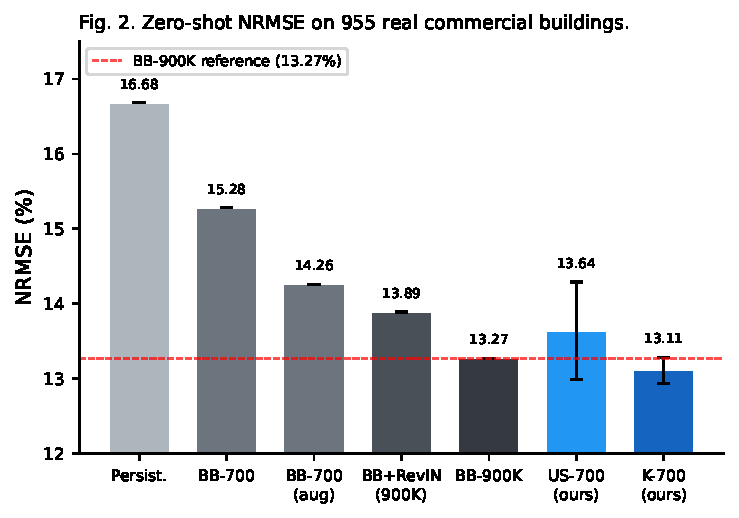
\includegraphics[width=0.75\textwidth]{figures/fig2_main_results.pdf}
\caption{Zero-shot NRMSE on 955 real commercial buildings. K-700 (ours) achieves 13.11\%, comparable to the BB-900K reference (13.27\%) with $1/1286$ the buildings. Error bars show five-seed standard deviation where available.}
\label{fig:main}
\end{figure}

\begin{table}[htbp]
\caption{External zero-shot validation on real commercial buildings (955-building evaluation set). Korean-700 and US-TMY-700 report five-seed mean $\pm$ std; Korean-700 (no aug) and Korean-700 (RevIN OFF) report three-seed mean $\pm$ std; all other rows use seed = 42. BB denotes the BuildingsBench stock-model corpus \citep{Emami2023}.}
\label{tab:main}
\centering
\small
\begin{tabular}{llllccccc}
\toprule
Model & Role & Data & N & RevIN & Aug & NRMSE (\%) & NCRPS (\%) & $\Delta$ \\
\midrule
\textbf{K-700} & \textbf{Proposed} & \textbf{LHS sim} & \textbf{700} & \textbf{ON} & \textbf{ON} & \textbf{13.11 $\pm$ 0.17} & \textbf{7.14 $\pm$ 0.03} & \textbf{$-$0.16} \\
\textbf{US-700} & \textbf{Weather abl.} & \textbf{US TMY} & \textbf{700} & \textbf{ON} & \textbf{ON} & \textbf{13.64 $\pm$ 0.65} & \textbf{7.53 $\pm$ 0.41} & \textbf{+0.37} \\
K-700 no aug & Aug ablation & LHS sim & 700 & ON & OFF & 13.67 $\pm$ 0.21 & 8.16 & +0.40 \\
K-700 no RevIN & RevIN abl. & LHS sim & 700 & OFF & ON & 14.72 $\pm$ 0.28 & 8.29 & +1.45 \\
BB-700 aug & Equal-size & BB subset & 700 & ON & ON & 14.26 & 7.80 & +0.99 \\
BB-700 & Control & BB subset & 700 & ON & OFF & 15.28 & --- & +2.01 \\
BB-900K & Ext. ref. & BB 900K & 900K & OFF & OFF & 13.27 & --- & --- \\
BB+RevIN & Ref.+RevIN & BB 900K & 900K & ON & OFF & 13.89 & 7.76 & +0.62 \\
Persist. & Naive & --- & --- & --- & --- & 16.68 & --- & +3.41 \\
\bottomrule
\end{tabular}
\end{table}

Under matched conditions (same architecture, optimizer, augmentation, number of buildings, and RevIN), the LHS-designed corpus outperforms the stock-model sample by \textbf{1.33 pp} at seed 42 (12.93\% vs.\ 14.26\%). The equal-scale BB-700 comparison uses a single stock-model subset and a single training seed, and therefore does not quantify subset-selection uncertainty. The 1.33 pp advantage should be interpreted as evidence from a controlled but not fully repeated comparison: the gap is substantially larger than the observed inter-seed variation of Korean-700 ($\pm$0.17 pp), but a definitive claim would require evaluating multiple BB-700 subsets across multiple seeds. The primary remaining difference is the design and source of the training data, although uncontrolled factors such as building codes, envelope properties, and climate mapping cannot be fully excluded (Section~\ref{sec:ablation}).

As a secondary observation, the designed dataset achieves performance comparable to the large stock-model reference (five-seed mean 13.11 $\pm$ 0.17\% vs.\ 13.27\%) without geographic metadata. A paired per-building comparison shows Korean-700 achieves lower error on 680 of 955 buildings (71\%); the paired bootstrap 95\% CI of the median per-building difference, defined as NRMSE(BB-900K) $-$ NRMSE(K-700), is [0.31, 0.39] pp using the seed-42 K-700 checkpoint (Wilcoxon signed-rank $p < 0.001$).

\subsection{Weather-Origin Ablation}
\label{sec:weather}

To test whether the observed benefit depends on the Korean weather files, we retrained on the same 700 LHS-designed buildings using U.S. TMY weather. The five-seed mean of US-TMY-700 is 13.64 $\pm$ 0.65\%, within 0.53 pp of Korean-700. The U.S.-TMY model still outperforms the equal-scale stock-model control (14.26\%) by 0.62 pp, suggesting that schedule design remains beneficial after replacing the Korean weather files.

\subsection{N-Scaling: Evidence for Coverage Saturation (Prediction 2)}
\label{sec:nscaling}

If the Operational Diversity Hypothesis is correct, performance should show diminishing returns once the LHS parameter space is adequately covered. Table~\ref{tab:nscaling} and Fig.~\ref{fig:nscaling} test this prediction.

\begin{figure}[htbp]
\centering
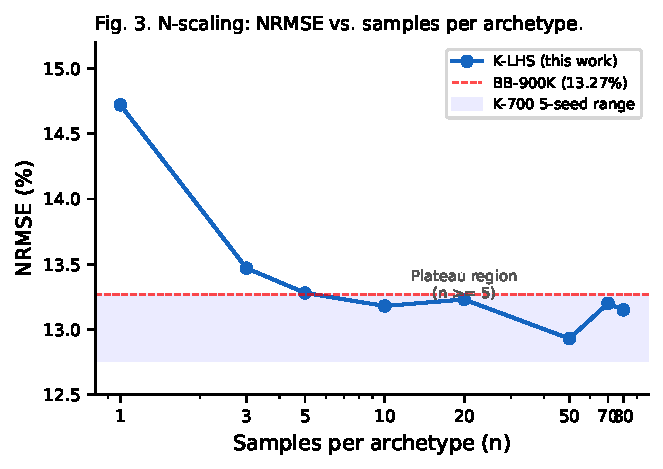
\includegraphics[width=0.65\textwidth]{figures/fig3_nscaling.pdf}
\caption{N-scaling: NRMSE vs.\ samples per archetype under a fixed 18,000-step training budget. Performance plateaus near the BB-900K reference level from $n \approx 5$ onward, consistent with the coverage-based interpretation.}
\label{fig:nscaling}
\end{figure}

\begin{table}[htbp]
\caption{N-scaling results (Transformer-M, RevIN ON, aug ON, $s = 18{,}000$, seed = 42). Exception: $n = 5$ reports five-seed mean $\pm$ std.}
\label{tab:nscaling}
\centering
\begin{tabular}{ccc}
\toprule
$n$ (per archetype) & Total Buildings & NRMSE (\%) \\
\midrule
1 & 14 & 14.72 \\
3 & 42 & 13.47 \\
5 & 70 & 13.28 $\pm$ 0.12 \\
10 & 140 & 13.18 \\
20 & 280 & 13.23 \\
50 & 700 & 12.93 \\
70 & 980 & 13.20 \\
80 & 1,120 & 13.15 \\
\bottomrule
\end{tabular}
\end{table}

Under the fixed 18,000-step training budget, performance improves sharply from $n = 1$ to $n = 5$ (14.72\% to 13.28\%), plateauing near the external reference level (13.27\%) from $n \approx 5$ onward. This early saturation is consistent with --- but does not by itself prove --- a coverage-based explanation. In a 12-dimensional schedule space, the covering radius decreases heuristically as $n^{-1/12}$, so doubling $n$ reduces $\varepsilon^*$ by only ${\sim}6\%$. However, we note that the fixed training budget means per-building exposure also changes with $n$, so the plateau reflects the joint effect of coverage saturation and optimization budget allocation.

The contrast with stock-model scaling is instructive (Appendix B): increasing from 700 to 7,000 stock-model buildings improves NRMSE by only 0.78 pp (15.28\% to 14.50\%), and even 7,000 stock-model buildings do not approach 700 LHS-designed buildings (13.11\%).

\subsection{Illustrative Coverage Proxy}
\label{sec:coverage_proxy}

To connect the conceptual framework with the performance comparisons, we compute an illustrative coverage proxy for the K-700 LHS design in the 12-dimensional normalized parameter space $[0,1]^{12}$. For a point set $S$, the proxy covering radius is estimated as $\varepsilon^*(S) = \max_{x \in T} \min_{s \in S} \|x - s\|_2$, where $T$ is a set of $10^5$ uniformly sampled test points. This analysis is descriptive: it compares LHS with simple synthetic reference samplers, not with the full BuildingsBench generation process.

\begin{table}[htbp]
\caption{Covering radius comparison in $[0,1]^{12}$ ($n = 50$ points per method, $10^5$ test points).}
\label{tab:coverage}
\centering
\begin{tabular}{lccc}
\toprule
Sampling Method & Mean distance & $\varepsilon^*$ (max) & $\varepsilon^*$ ratio vs.\ LHS \\
\midrule
K-700 LHS & 0.862 & 1.399 & 1.00 \\
Random Uniform & 0.854 & 1.412 & 1.01 \\
Clustered (stock-model proxy) & 1.089 & 1.985 & 1.42 \\
\bottomrule
\end{tabular}
\end{table}

The clustered set simulates a concentrated sampler by drawing 50 points from $\mathcal{N}(\mu_{\text{typical}}, 0.15I)$ clipped to $[0,1]^{12}$. Its proxy covering radius is 42\% larger than LHS, meaning that in this illustrative setup the worst-case target point lies farther from the nearest training sample. We treat this result only as intuition for why broader sampling can help; it is not a direct measurement of BuildingsBench coverage.

\textbf{Feature-space proximity does not explain the gain.} To complement the design-parameter analysis, we also compare K-700 and BB-700 in an 8-dimensional \emph{time-series feature space} derived from the actual hourly load profiles: night/day ratio, weekend/weekday ratio, daily-peak CV, operating hours, morning ramp rate, weekly autocorrelation (lag-168), seasonality CV, and baseload fraction. For each of K-700, BB-700, and the 955 real evaluation buildings, we extract these features and normalize jointly to $[0,1]^8$.

\begin{table}[htbp]
\caption{Feature-space proximity to real buildings. Mean NN distance from each of the 955 real evaluation buildings to the nearest point in the training dataset (lower = closer to real). MMD: Maximum Mean Discrepancy with RBF kernel.}
\label{tab:feature_coverage}
\centering
\begin{tabular}{lcccc}
\toprule
Dataset & Mean NN & P95 NN & \% within $d < 0.2$ & MMD to Real \\
\midrule
K-700 & 0.148 & 0.413 & 78.9\% & 0.609 \\
BB-700 & 0.109 & 0.251 & 92.0\% & 0.498 \\
\bottomrule
\end{tabular}
\end{table}

Table~\ref{tab:feature_coverage} reveals that BB-700 lies \emph{closer} to real buildings in feature space than K-700: its mean nearest-neighbor distance is 26\% smaller, and 92\% of real buildings have a BB-700 neighbor within $d = 0.2$ versus 79\% for K-700. Per-feature analysis confirms this pattern: BB-700 covers 76\% of the real operating-hours range and 84\% of the weekly-autocorrelation range, whereas K-700 covers only 42\% and 23\%, respectively. The narrow K-700 operating-hours range reflects high baseload and nighttime equipment fractions in many LHS samples, which cause the feature extractor to classify them as near-continuous operation even when the \texttt{op\_duration} parameter spans 8--24 h.

This result clarifies what ``coverage'' means in the context of zero-shot transfer. K-700 achieves superior forecasting accuracy (Table~\ref{tab:main}) \emph{despite} covering a narrower region of the observed feature distribution. The benefit of LHS is therefore not explained by closer marginal feature matching to the real-building distribution. Rather, LHS acts as a \emph{structured intervention over operational factors}, creating disentangled temporal-pattern variation that teaches the model robust pattern decomposition across the designed operational parameter space---including extreme combinations that rarely occur in real stocks. RevIN then bridges the remaining distributional gap at inference time by removing building-specific magnitude and variability. This interpretation is consistent with Prediction~3: RevIN's benefit is largest precisely when the training data's feature distribution differs most from the target distribution.

\subsection{Ablation Studies (Prediction 3)}
\label{sec:ablation}

Table~\ref{tab:ablation} reports ablations for RevIN and geographic metadata.

\begin{table}[htbp]
\caption{Ablation results (seed 42, checkpoint selected on held-out simulation validation set, evaluated on the 955 real-building test set). The validation set consists of withheld simulation buildings and does not overlap with the 955-building evaluation set.}
\label{tab:ablation}
\centering
\begin{tabular}{lcc}
\toprule
Experiment & NRMSE (\%) & $\Delta$ \\
\midrule
K-700 RevIN ON (baseline) & 12.93 & --- \\
K-700 RevIN OFF & 14.81 & +1.88 \\
Actual lat/lon coordinates & 12.93 & 0.00 \\
\bottomrule
\end{tabular}
\end{table}

Exploratory runs from an earlier pipeline iteration are reported in Appendix~C for transparency. These runs---using stock-model-fitted Box-Cox parameters, extended training, scaling to 70K buildings, and seasonal decomposition before RevIN---all degraded performance, but because they were conducted under a different pipeline configuration, they are not used as primary evidence for the claims in this paper.

%% ============================================================
\section{Discussion}
\label{sec:discussion}

\subsection{Mechanistic Interpretation of RevIN's Regime-Dependent Effect (Prediction 3)}

The asymmetry in RevIN's effect across dataset scales (Fig.~\ref{fig:revin}) admits a coherent mechanistic interpretation that extends beyond our specific setting.

\begin{figure}[htbp]
\centering
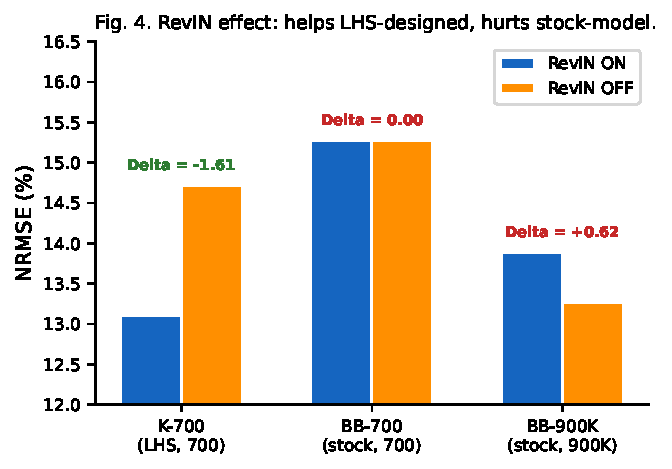
\includegraphics[width=0.65\textwidth]{figures/fig4_revin_effect.pdf}
\caption{RevIN's regime-dependent effect. RevIN improves K-700 (LHS-designed, $\Delta = -1.61$ pp) but degrades BB-900K (stock-model, $\Delta = +0.62$ pp), consistent with the scale-shape independence assumption (A3). K-700 values use five-seed means from Table~\ref{tab:main}; the seed-42 ablation in Table~\ref{tab:ablation} shows a larger single-seed delta of $-1.88$ pp.}
\label{fig:revin}
\end{figure}

RevIN normalizes each context window to zero mean and unit variance, stripping absolute load magnitude. With a small LHS-designed dataset, the model has not seen enough magnitude variation to internalize it; RevIN reduces this burden by normalizing instance-level scale and variability, yielding a substantial improvement (Table~\ref{tab:ablation}). With a large stock-model corpus---where each building contributes only a few training windows---magnitude may carry transferable information because it is correlated with building type, HVAC configuration, and schedule assumptions in the generation pipeline. Removing this information may discard something useful, producing a measurable degradation (Table~\ref{tab:main}).

A structural factor reinforces this. In stock-model corpora, magnitude is informative about building type because HVAC, envelope, and schedule are jointly determined by the generation pipeline---magnitude and temporal shape are correlated. In our LHS design, magnitude reflects only the scale\_mult parameter, sampled independently of schedule parameters. RevIN's removal of magnitude therefore discards less useful information in LHS data than in stock-model data.

This finding has implications for the broader time series community: RevIN's benefit depends not just on dataset size but on the information structure of the training data---specifically, whether magnitude carries predictive information about temporal dynamics.

\subsection{Design Principles Behind Transferable Pattern Coverage}

The methodology's effectiveness can be traced to three design principles:

\begin{enumerate}
\item \textbf{Independent marginal coverage through LHS.} Each of the 12 schedule parameters is sampled with uniform marginal coverage, ensuring that the training set visits the full range of each operational dimension---including extreme combinations that rarely occur in real building stocks but expose the model to temporal dynamics it must handle at inference time.

\item \textbf{Archetype-stratified diversity.} Stratifying the 12D LHS across 14 building archetypes ensures that schedule diversity interacts with distinct thermal mass, HVAC response, and internal gain profiles. This produces a combinatorial expansion of temporal patterns: the same nighttime equipment retention fraction yields qualitatively different load shapes in a hospital versus a strip mall.

\item \textbf{Decoupled magnitude and temporal shape.} The scale\_mult parameter is sampled independently of the 11 schedule parameters, reducing the extent to which load magnitude encodes schedule-driven temporal dynamics. This structural property helps explain why RevIN helps in our design but hurts in stock-model corpora.
\end{enumerate}

\subsection{Practical Implications}

The reframing from scale to design has immediate practical consequences. An organization can generate several hundred parametric EnergyPlus simulations conforming to local building codes and climate, train a standard Transformer with RevIN and augmentation, and deploy zero-shot forecasting---without assembling a national building stock database.

The computational cost is modest: 700 simulations completed in approximately 4 hours on a single workstation (10-core CPU, 64 GB RAM); training takes approximately 2 hours on a single consumer GPU (NVIDIA RTX 4090). The entire pipeline from simulation to deployed model takes less than a day.

\subsection{Limitations (Including Prediction 4)}
\label{sec:limitations}

Our parametric simulations differ from the stock-model baseline in schedule design, climate, building codes, and envelope parameters. The equal-scale controlled experiment controls for augmentation, model architecture, and training budget, but cannot fully disentangle all data-source-related confounds. The U.S.-TMY ablation substantially reduces but does not eliminate the climate-origin confound.

The equal-scale BB-700 comparison uses a single stock-model subset with a single training seed. Repeating this comparison across multiple subsets and seeds would strengthen the claim but requires approximately 50 hours of additional training; we leave this for future work. The 1.33 pp advantage over BB-700 should therefore be interpreted cautiously.

The objective of this study is not to claim a large performance breakthrough, but to demonstrate that a systematically designed simulation dataset can provide competitive zero-shot transfer with substantially lower data requirements. The margin between the designed dataset and the large-scale reference is comparable to inter-seed variation. The contribution is methodological: showing that systematic simulation design can substantially reduce reliance on brute-force dataset scaling.

All experiments use a single model architecture (Transformer-M); generalization to PatchTST, MOIRAI, or other architectures has not been tested.

The coverage-based framework in Section~\ref{sec:framework} is deliberately simplified. It is useful for interpreting the results, but it does not estimate the true target distribution, prove asymptotic rates for the actual benchmark pipeline, or directly measure the coverage of BuildingsBench itself.

On residential buildings, our model yields accuracy comparable to the Persistence Ensemble. The framework of Section~\ref{sec:framework} suggests that this is a coverage gap: residential buildings occupy a parameter space $\Theta_{\text{res}}$ that is largely disjoint from the commercial space $\Theta_{\text{com}}$ used for training. Extending the approach to residential buildings therefore requires a separate $\Theta_{\text{res}}$ with residential-specific schedule parameters.

%% ============================================================
\section{Conclusion}
\label{sec:conclusion}

We presented a coverage-based interpretation of the Operational Diversity Hypothesis for zero-shot building load forecasting. The central claim is practical rather than absolute: a compact simulation dataset can remain competitive when it is designed to span diverse operating regimes instead of merely increasing sample count. Controlled experiments are broadly consistent with this interpretation:

(1) in the single-subset equal-scale control, the LHS-designed dataset outperforms the BB-700 stock-model sample (12.93\% vs.\ 14.26\% NRMSE) under matched training conditions; (2) N-scaling plateaus around $n \approx 5$ per archetype under the fixed training budget used here; (3) RevIN reduces NRMSE by 1.88 pp on LHS data but increases it by 0.62 pp on stock-model data, consistent with differences in how magnitude information is structured; and (4) residential forecasting remains weak when training covers only commercial operating regimes.

Taken together, the results suggest that the data requirement for zero-shot building energy forecasting should be framed partly as a structured parameter-intervention problem, not only as a scale problem. Feature-space analysis (Table~\ref{tab:feature_coverage}) confirms that the benefit does not arise from closer distributional matching to real buildings; rather, LHS acts as a disentangled intervention over operational factors that teaches robust pattern decomposition. A dataset of 700 simulations designed for broad operational-factor variation achieves transfer performance comparable to a 900K-building stock-model corpus, reducing the entire pipeline to less than a day on a single workstation.

The principal open questions are extending the framework to residential buildings, testing generalization across model architectures (PatchTST, MOIRAI), measuring coverage more directly against real and stock-model datasets, and resolving the augmentation asymmetry between training pipelines.

%% ============================================================
\section*{CRediT authorship contribution statement}
\textbf{Jeong-Uk Kim:} Conceptualization, Methodology, Software, Validation, Formal analysis, Investigation, Data curation, Writing -- original draft, Visualization.

\section*{Declaration of competing interest}
The author declares that there is no known competing financial interest or personal relationship that could have appeared to influence the work reported in this paper.

\section*{Declaration of generative AI in scientific writing}
During the preparation of this work, the author used large language models (Claude, GPT-4) for literature search assistance, writing refinement, and code debugging. The author reviewed and edited all outputs and takes full responsibility for the content of the publication.

\section*{Data availability}
The LHS parameter configurations, EnergyPlus IDF templates, evaluation scripts, and trained model checkpoints will be made available via a public GitHub repository upon acceptance. An anonymized repository containing these materials will be provided for peer review.

\section*{Acknowledgements}
This work was supported by internal research funds from Sangmyung University.

\bibliographystyle{elsarticle-harv}
\bibliography{references}

%% ============================================================
\appendix

\section{Multi-Seed Results}
\label{app:seeds}

\subsection{Korean-700 RevIN ON ($s = 18{,}000$, 5 seeds)}

\begin{table}[H]
\centering
\begin{tabular}{ccc}
\toprule
Seed & NRMSE (\%) & NCRPS (\%) \\
\midrule
42 & 12.93 & 7.10 \\
43 & 13.06 & 7.16 \\
44 & 13.10 & 7.16 \\
45 & 13.39 & n.e. \\
46 & 13.07 & 7.14 \\
\textbf{Mean $\pm$ Std} & \textbf{13.11 $\pm$ 0.17} & \textbf{7.14 $\pm$ 0.03}$^\dagger$ \\
\bottomrule
\end{tabular}
\caption{Five-seed results for Korean-700 (RevIN ON, augmentation ON). $^\dagger$Four-seed NCRPS mean (seeds 42, 43, 44, 46); seed 45 NCRPS not evaluated with the retrained checkpoint.}
\label{tab:seeds_on}
\end{table}

\subsection{Korean-700 RevIN OFF ($s = 18{,}000$, 3 seeds)}

\begin{table}[H]
\centering
\begin{tabular}{ccc}
\toprule
Seed & NRMSE (\%) & NCRPS (\%) \\
\midrule
42 & 14.81 & 8.17 \\
43 & 14.94 & n.e. \\
44 & 14.40 & 8.40 \\
\textbf{Mean $\pm$ Std} & \textbf{14.72 $\pm$ 0.28} & \textbf{8.29}$^\ddagger$ \\
\bottomrule
\end{tabular}
\caption{Three-seed results for Korean-700 (RevIN OFF). $^\ddagger$Two-seed NCRPS mean (seeds 42, 44).}
\label{tab:seeds_off}
\end{table}

\subsection{Korean-700 RevIN ON ($s = 16{,}000$, 5 seeds)}

Five-seed evaluation at $s = 16{,}000$ yields $13.13 \pm 0.15\%$, confirming robustness to training duration.

\begin{table}[H]
\centering
\begin{tabular}{cc}
\toprule
Seed & NRMSE (\%) \\
\midrule
42 & 12.89 \\
43 & 13.24 \\
44 & 13.16 \\
45 & 13.26 \\
46 & 13.12 \\
\textbf{Mean $\pm$ Std} & \textbf{13.13 $\pm$ 0.15} \\
\bottomrule
\end{tabular}
\caption{Five-seed results at $s = 16{,}000$ training steps.}
\label{tab:seeds_16k}
\end{table}

\subsection{Korean-700 No Augmentation ($s = 18{,}000$, 3 seeds)}

\begin{table}[H]
\centering
\begin{tabular}{ccc}
\toprule
Seed & NRMSE (\%) & NCRPS (\%) \\
\midrule
42 & 13.48 & 7.95 \\
43 & 13.89 & 8.21 \\
44 & 13.65 & 8.31 \\
\textbf{Mean $\pm$ Std} & \textbf{13.67 $\pm$ 0.21} & \textbf{8.16 $\pm$ 0.18} \\
\bottomrule
\end{tabular}
\caption{Three-seed results without data augmentation.}
\label{tab:seeds_noaug}
\end{table}

\subsection{Stock-Model 900K + RevIN}

The 900K stock-model baseline retrained with RevIN achieves 13.89\%, a 0.62 pp degradation relative to the original 13.27\%.

\FloatBarrier
\section{Stock-Model Scaling (700 and 7,000 Buildings)}
\label{app:scaling}

\begin{table}[H]
\centering
\begin{tabular}{lcccc}
\toprule
Configuration & $N$ & RevIN & Aug & NRMSE (\%) \\
\midrule
Stock-700 & 700 & ON & OFF & 15.28 \\
Stock-700 (aug) & 700 & ON & ON & 14.26 \\
Stock-700 & 700 & OFF & OFF & 16.44 \\
Stock-7K & 7,000 & ON & OFF & 14.50 \\
Stock-7K & 7,000 & OFF & OFF & 15.41 \\
\bottomrule
\end{tabular}
\caption{Stock-model scaling results. A 10$\times$ increase in stock-model buildings (700 to 7,000) reduces NRMSE by only 0.78 pp, and even 7,000 stock-model buildings (14.50\%) do not approach 700 LHS-designed buildings (13.11\%).}
\label{tab:stock_scaling}
\end{table}

\FloatBarrier
\section{Exploratory Ablation Results (Earlier Pipeline)}
\label{app:ablations}

\begin{table}[H]
\centering
\begin{tabular}{lccc}
\toprule
Experiment & NRMSE (\%) & $\Delta$ vs.\ baseline & Mechanism \\
\midrule
BB Box-Cox & 16.24 & +3.31 & Distribution mismatch \\
4$\times$ tokens (168K steps) & 16.02 & +3.09 & Synthetic overfitting \\
5K cap (70K buildings) & 15.35 & +2.42 & Fixed-budget undersampling \\
Seasonal decomp + RevIN & 16.65 & +3.72 & Periodicity disruption \\
\bottomrule
\end{tabular}
\caption{Exploratory ablations from an earlier pipeline iteration (seed 42), reported for transparency. These results are not directly comparable to the final pipeline and are not used as primary evidence. Baseline is K-700 at 12.93\%. $\Delta$ is NRMSE increase in percentage points.}
\label{tab:extra_ablations}
\end{table}

\end{document}
